\section{Introduction}
The International Linear Collider (ILC) is a proposed  
$\ee$ collider with a center of mass energy of up to 1 TeV
that will enable the particle physics community to perform 
precision studies of the Higgs boson
and search for physics beyond
 the Standard Model~\cite{Baer:2013cma}.
The  physics goals of the ILC
 necessitate the development of collider detectors with unprecedented 
%performance, including
charged particle tracking capabilities~\cite{Behnke:2013lya}.
%In comparison to the LHC,
%the ILC's relatively gentle beam environment
%in comparison to the LHC
%permits detector designs with minimal material
%budgets in the tracker volumes~\citeBehnke:2013lya}.
Two different detector designs have been put forward
for the ILC, the International Large Detector~(ILD)
and the Silicon Detector~(SiD).
ILD uses a time projection chamber to provide
continuous charged particle tracking and a very low material budget
between the interaction point and the calorimeter~\cite{Behnke:2013lya}.
SiD uses all-silicon tracking in a 5~Tesla magnetic field,
resulting in a compact and cost-controlled detector
that has excellent tracking performance and 
can mitigate $\ee$ pair background~\cite{Behnke:2013lya}.
The ILC has been designed
 %to include the `push-pull' system, which allows
such that both detectors
alternately share the same interaction point via
the so-called ``push-pull'' system, in which
one detector slides out to accommodate the other~\cite{Behnke:2013lya}
%, providing
%experimental complementarity
% will be used alternately via the so-callled
%`push-pull' system 
%while sharing the same interaction point~\citeBehnke:2013lya}.

It is crucial that the design of the tracking system
be optimized with respect to various parameters,
including but not limited to material budgets,
segmentation ~\cite{2011arXiv1104.4547W},
and tracker geometry.
%in order to maximize performance.
%with respect to the various parameters by which collider detectors are constructed.
This paper presents tracking performance studies
%of a modified vertex detector geometry for the SiD
 optimizing the vertex detector
geometry of the SiD baseline design,
`Sidloi3' (figure~\ref{fig:trackersketch}), as presented in the SiD
detailed baseline document (DBD)~\cite{Behnke:2013lya}.
We first provide an overview of Sidloi3's tracking systems,
and then present the vertex barrel geometry
modification which was investigated.
We only modified the geometry of the
barrels of the vertex detector.
We then discuss our simulation, 
 reconstruction, and analysis methods and present
the tracking performance of the modified vertex barrel in
comparison to the tracking performance of the
Sidloi3 detector.

\section{Baseline Tracking System}
\begin{figure}
\centering
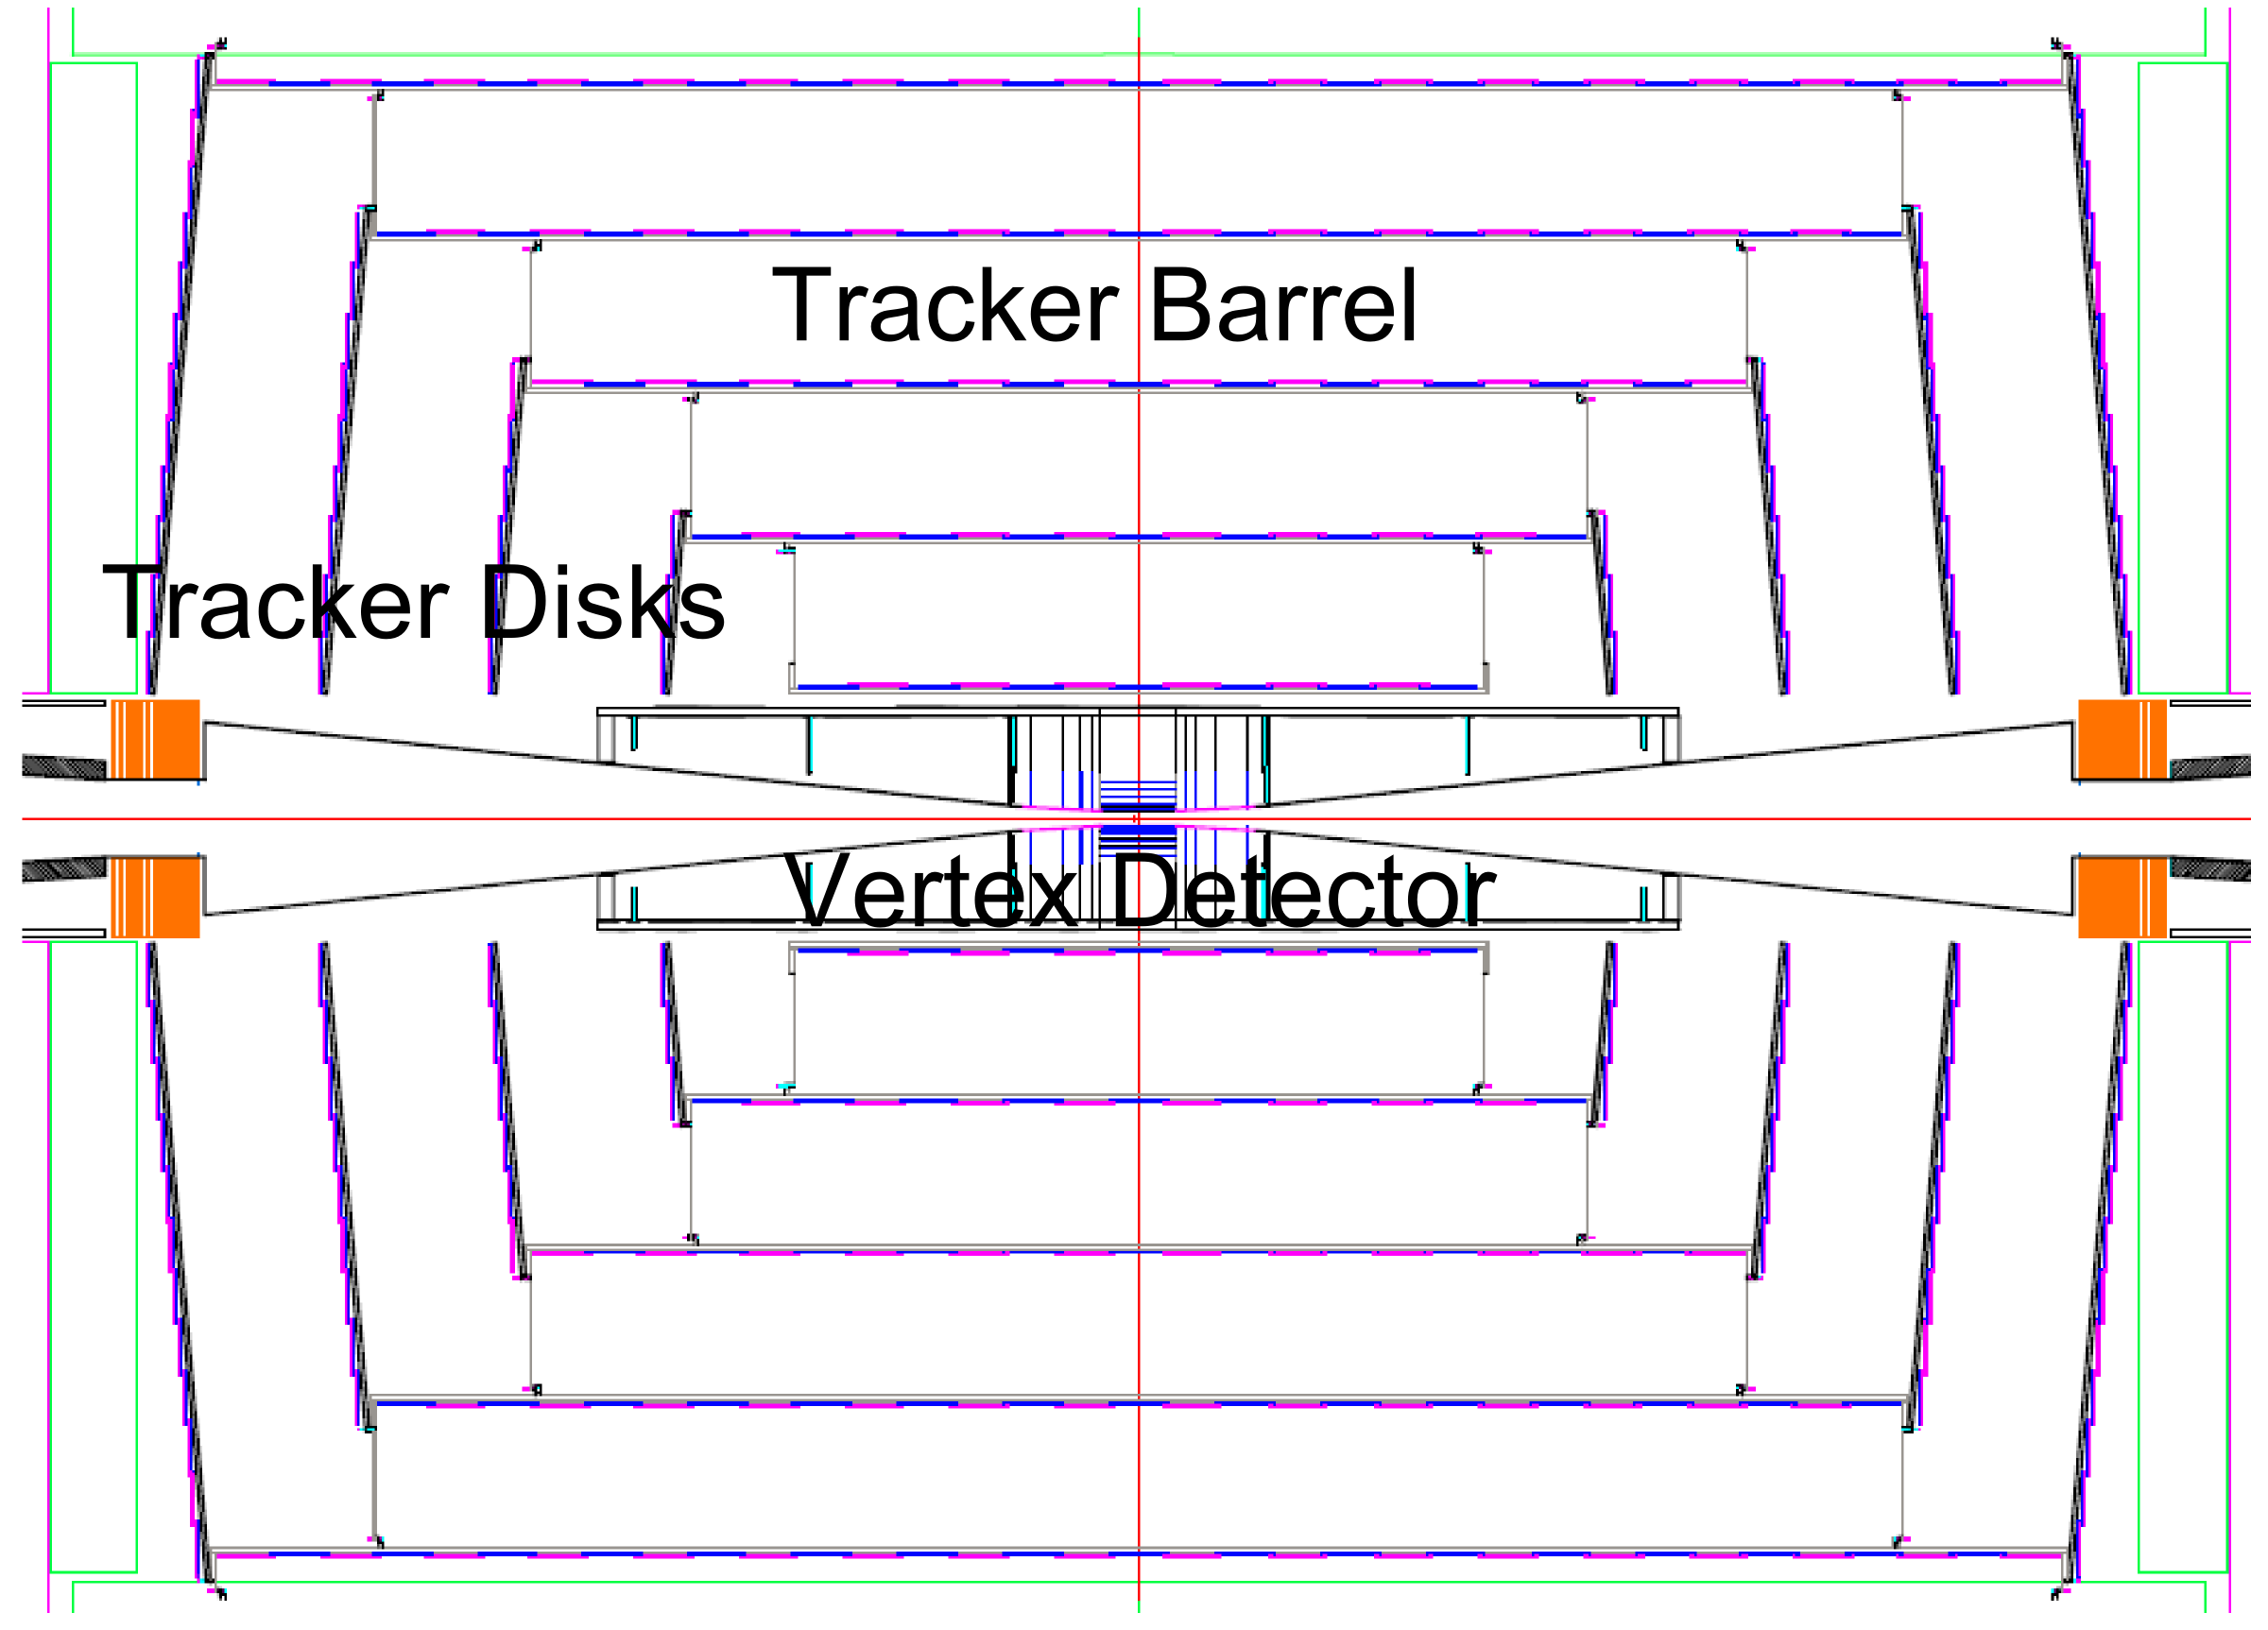
\includegraphics{totalTracker.png}
\caption{The entire Sidloi3 tracker. A more detailed sketch
of the vertex subdetectors is given in figure~\ref{fig:vertexsketch}.
The figure is taken from the SiD DBD~\cite{Behnke:2013lya}.}
\label{fig:trackersketch}
\end{figure}
The silicon single length crossing time stamping as implemented by 
Sidloi3 include robust handling of the ILC
 beam background and outstanding momentum resolution for charged particles~\cite{Behnke:2013lya}.
Sidloi3 uses all-silicon tracking with %a combination of
pixel segmentation in the vertex barrels and disks, 
and strip segmentation in the tracker barrels and disks~\cite{Behnke:2013lya}.
The entire tracker is shown in figure~\ref{fig:trackersketch} and
each subdetector's coverage as a function of polar angle is shown in figure~\ref{fig:coveragea}.
Details concerning the segmentation and readout dimensions 
used for this study may be found in section~\ref{sec:recon}.
%See figure \textbf{FIGURE} for an illustration of the various tracking systems in Sidloi3.
For a more detailed look at each of the tracking systems
as well as hardware and electronics research and development,
% including more detailed dimensions,
see~\cite{Behnke:2013lya}.

\subsection{Sidloi3 Baseline Vertex Detector}
\begin{figure}[t]
\centering
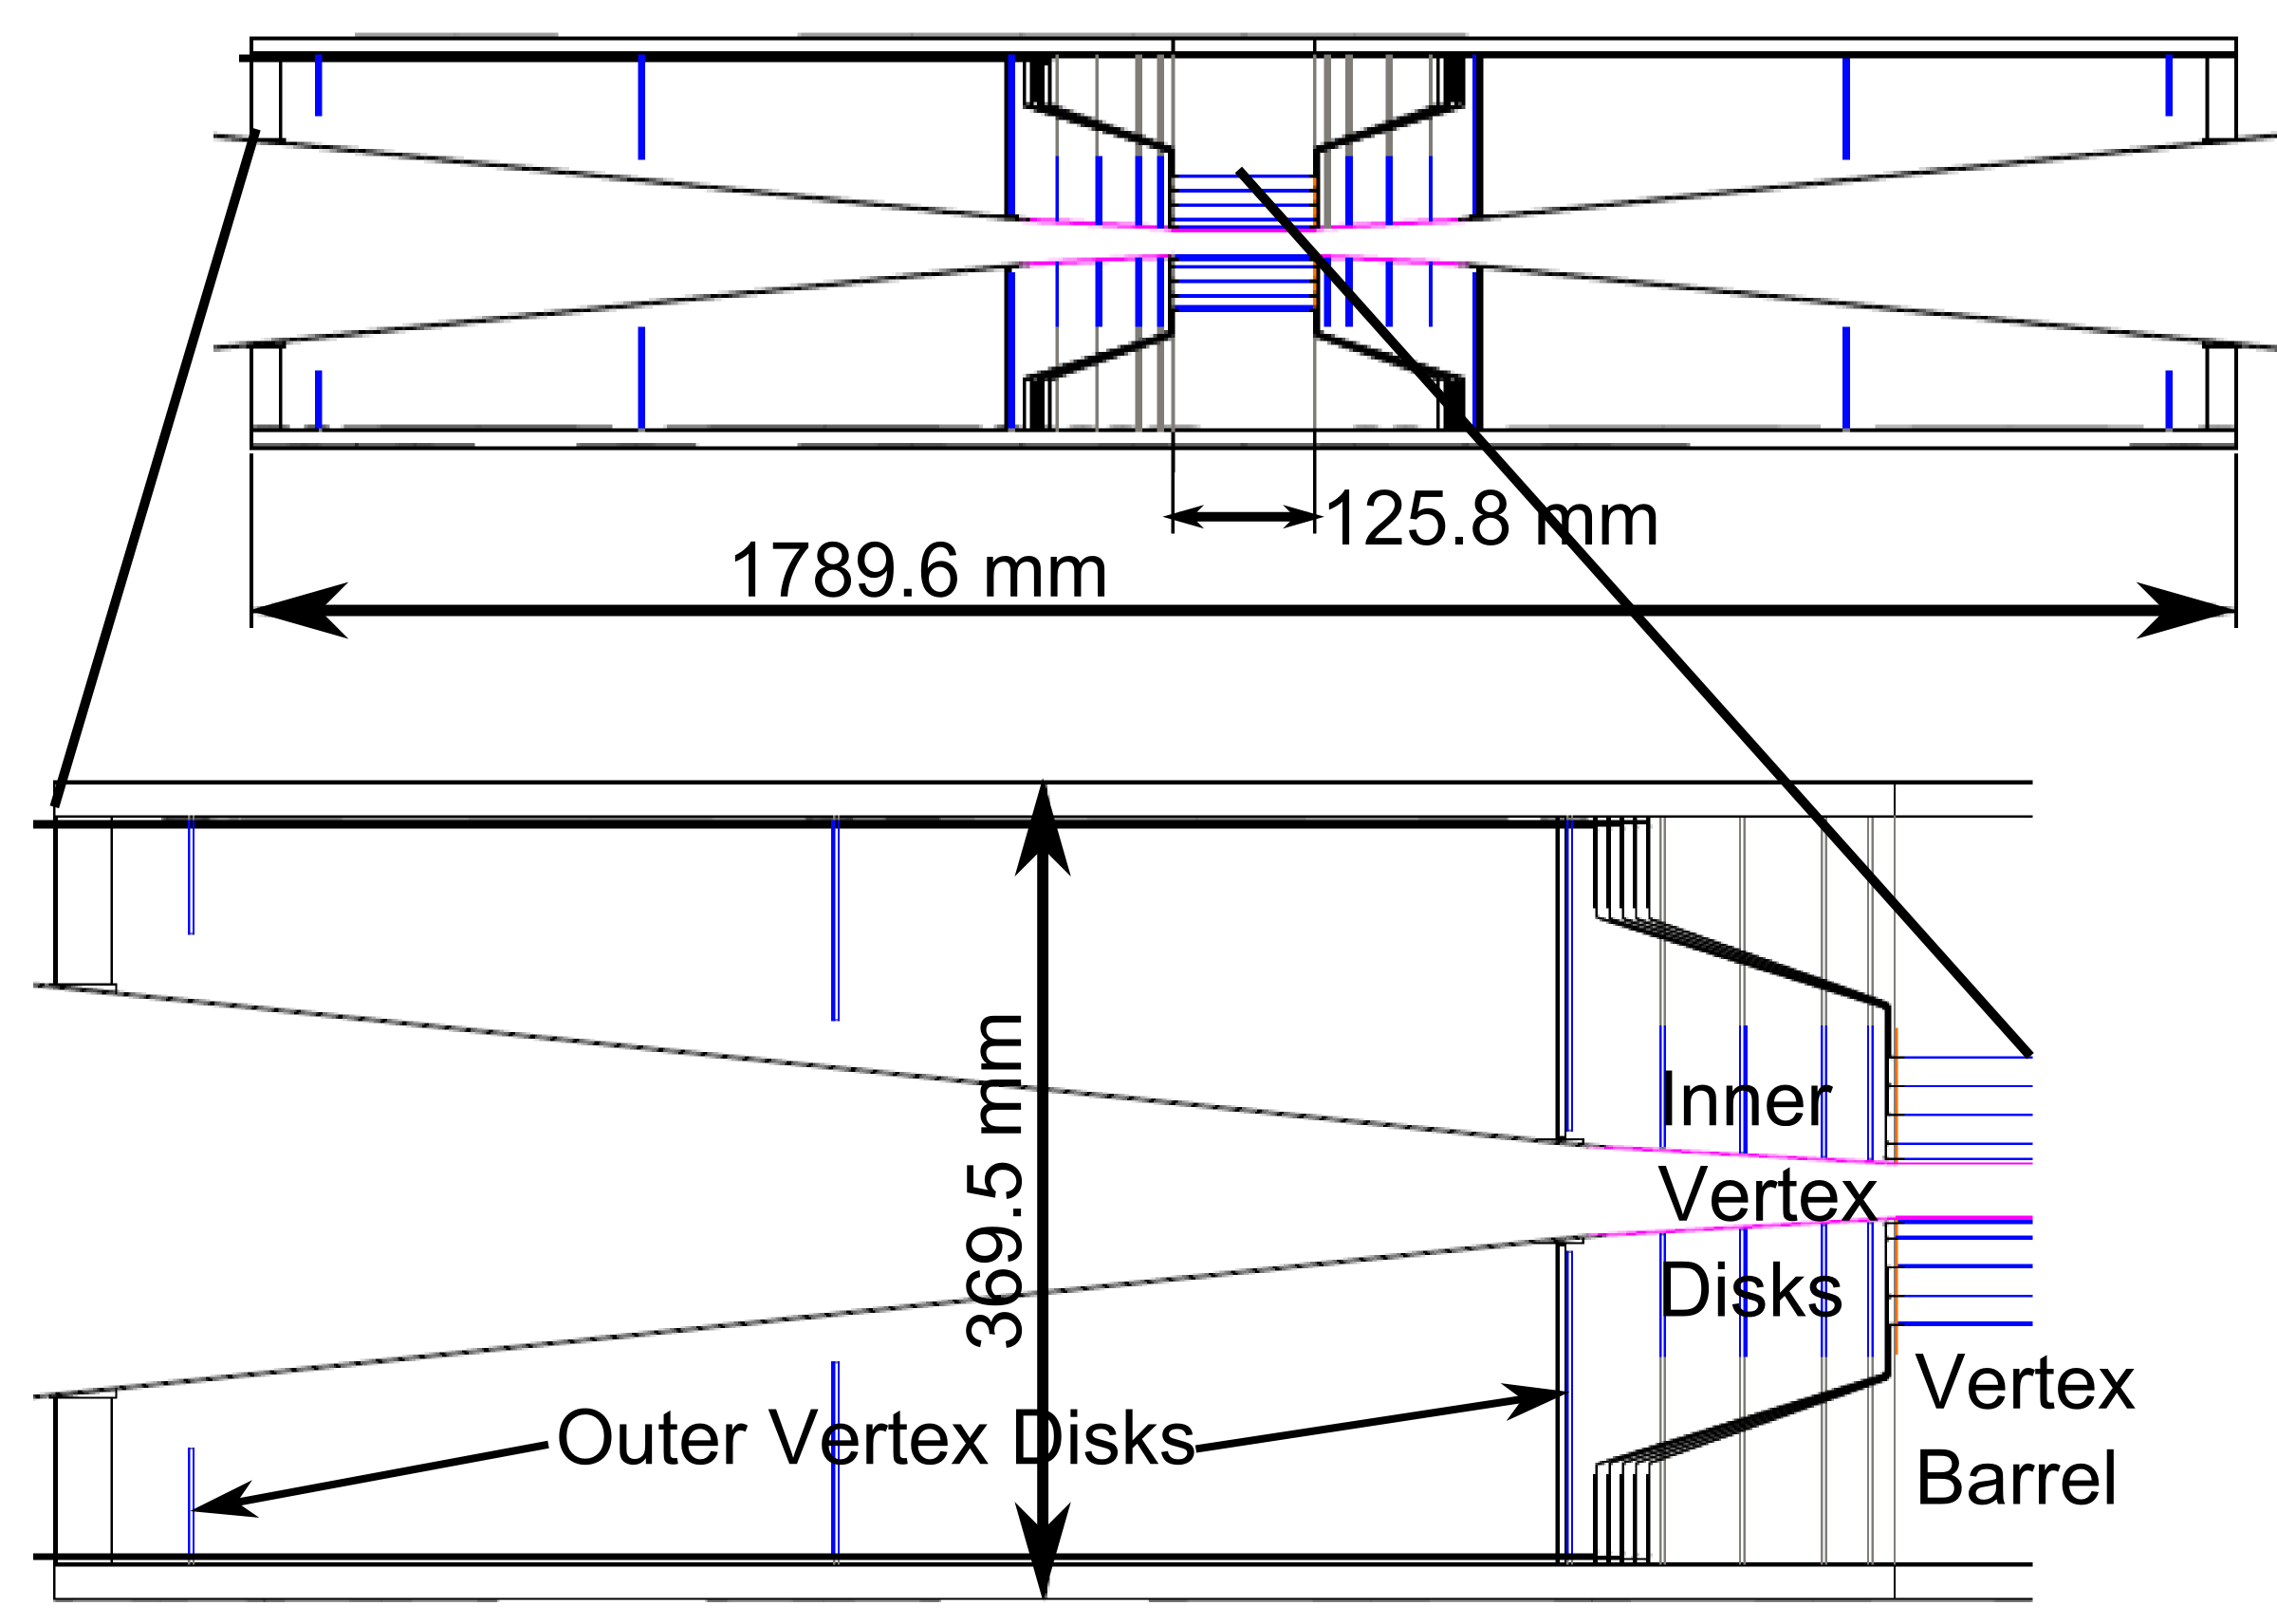
\includegraphics{vertexDetectorSketch1.png}
\caption{The vertex barrel, inner, and outer disks
in the Sidloi3 detector~\cite{Behnke:2013lya}.}
\label{fig:vertexsketch}
\end{figure}
The vertex detector of Sidloi3 (figure~\ref{fig:vertexsketch})
has been designed so as to have excellent tracking precision
and a very low material budget, to reduce the effects from multiple Coulomb scattering.
%In addition to a barrel,
Sidloi3's vertex detector includes barrel layers wrapping
around the interaction point,
inner disks close to the interaction point (small $z$),
and outer disks away from the interaction point (large $z$).
All tracking parts of the vertex detector feature $20 \times 20~\mu m^{2}$ pixel segmentation.
The vertex detector is arranged so as to provide 
broad coverage for a wide polar angle, $\cos{\theta} \approx 0.984$~\cite{Behnke:2013lya}.
The polar angle coverage of Sidloi3's vertex tracking systems
 is illustrated in figure~\ref{fig:coveragea}.
Note that figure~\ref{fig:coveragea} also includes
the coverage of the outer trackers (figure~\ref{fig:trackersketch}, which are further
from the interaction point than the vertex detectors.
%An illustration of the entire vertex detector in Sidloi3 is given in \textbf{ADD FIGURE}.

\subsection{Vertex Barrel Geometry Modification}
The Sidloi3 vertex barrel geometry consists of five pixellated layers, as illustrated in figure~\ref{fig:sidloi3barrel}.
The modified geometry that we studied consists of six such layers grouped into three sets of two ``doublet'' layers, 
as illustrated in figure~\ref{fig:modifiedbarrel}, with a gap of $3~mm$ between layers in each doublet.
Table~\ref{tab:vertexGeom} gives some of the geometry parameters of the two different radial barrels.
The modified geometry keeps layers one, three, and five in the same position as in Sidloi3.
The modified geometry also keeps the same thickness and segmentation
of the modules comprising the vertex barrel.
%thickness and segmentation of the modules comprising the barrels are both kept the same in the modified detector.
The width of the tracker module remains the same for most layers except layers two and four.
For two and four, the module is wider by $1$~mm in order to 
insure proper overlap at the module junctions at a greater radial distance from the interaction point.
%For those layers within each doublet of the modified geometry,
The $\phi$ rotation for detector modules and the number of modules
are kept the same for layers within each doublet.
No other modifications were made to the vertex barrel of Sidloi3 or to any other part of the Sidloi3 detector.
Figure~\ref{fig:coverage} illustrates the coverage of the tracking systems as a function of polar angle for both detectors.
Notice that the coverage for all tracking systems increased the number of hits
in the vertex detector at large angle.
%Figure~\ref{fig:coverage}(b) illustrates the coverage of the tracking systems in the modified detector as a function of polar angle.
\begin{figure}
\begin{minipage}{.5\textwidth}
\centering
%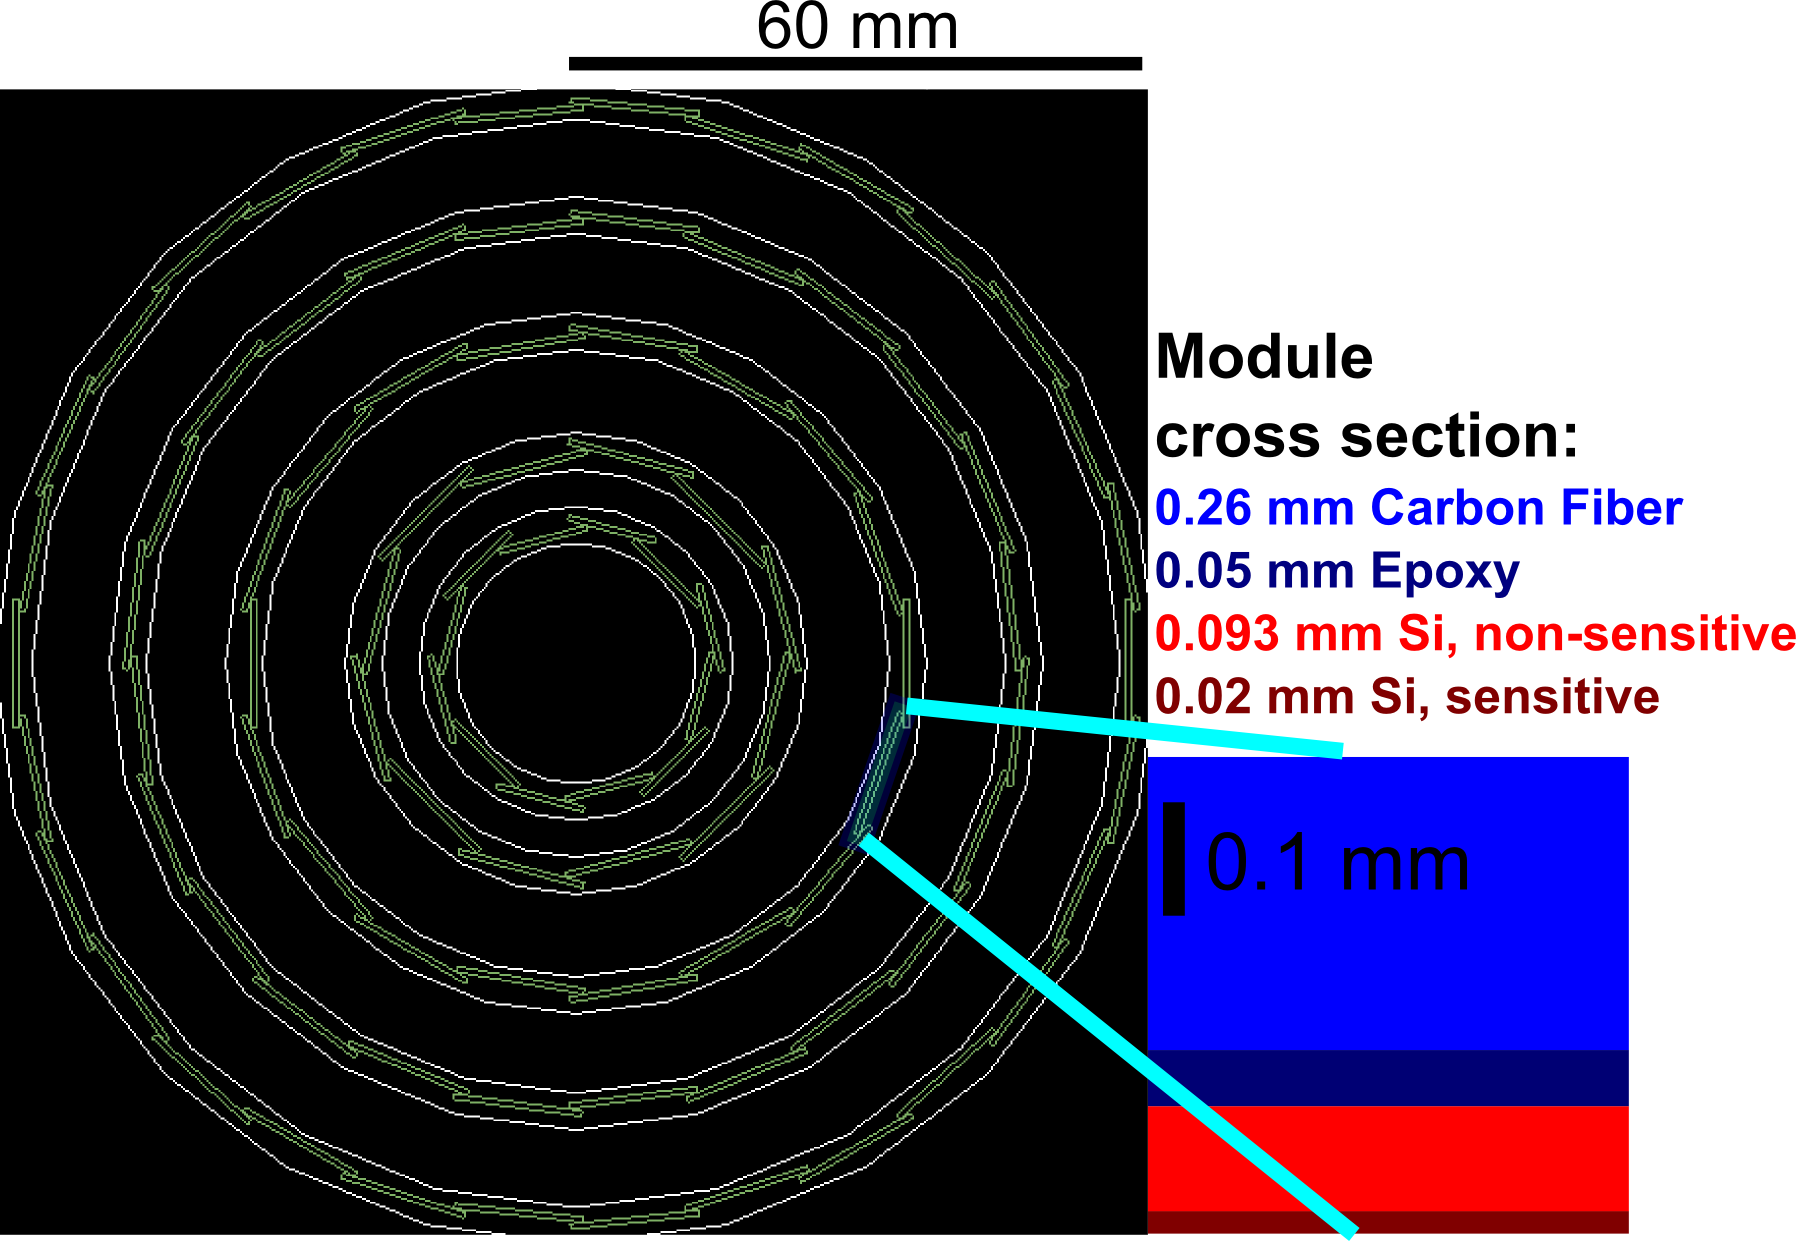
\includegraphics{sidloi3_barrel3.png}
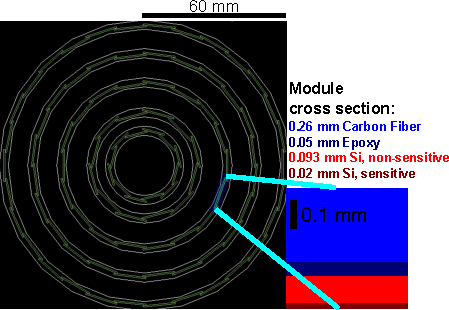
\includegraphics{sidloi3_barrel_withVolumes.pdf}
\subcaption{Sidloi3 Barrel}\label{fig:sidloi3barrel}
\end{minipage}%
\begin{minipage}{.5\textwidth}
\centering
%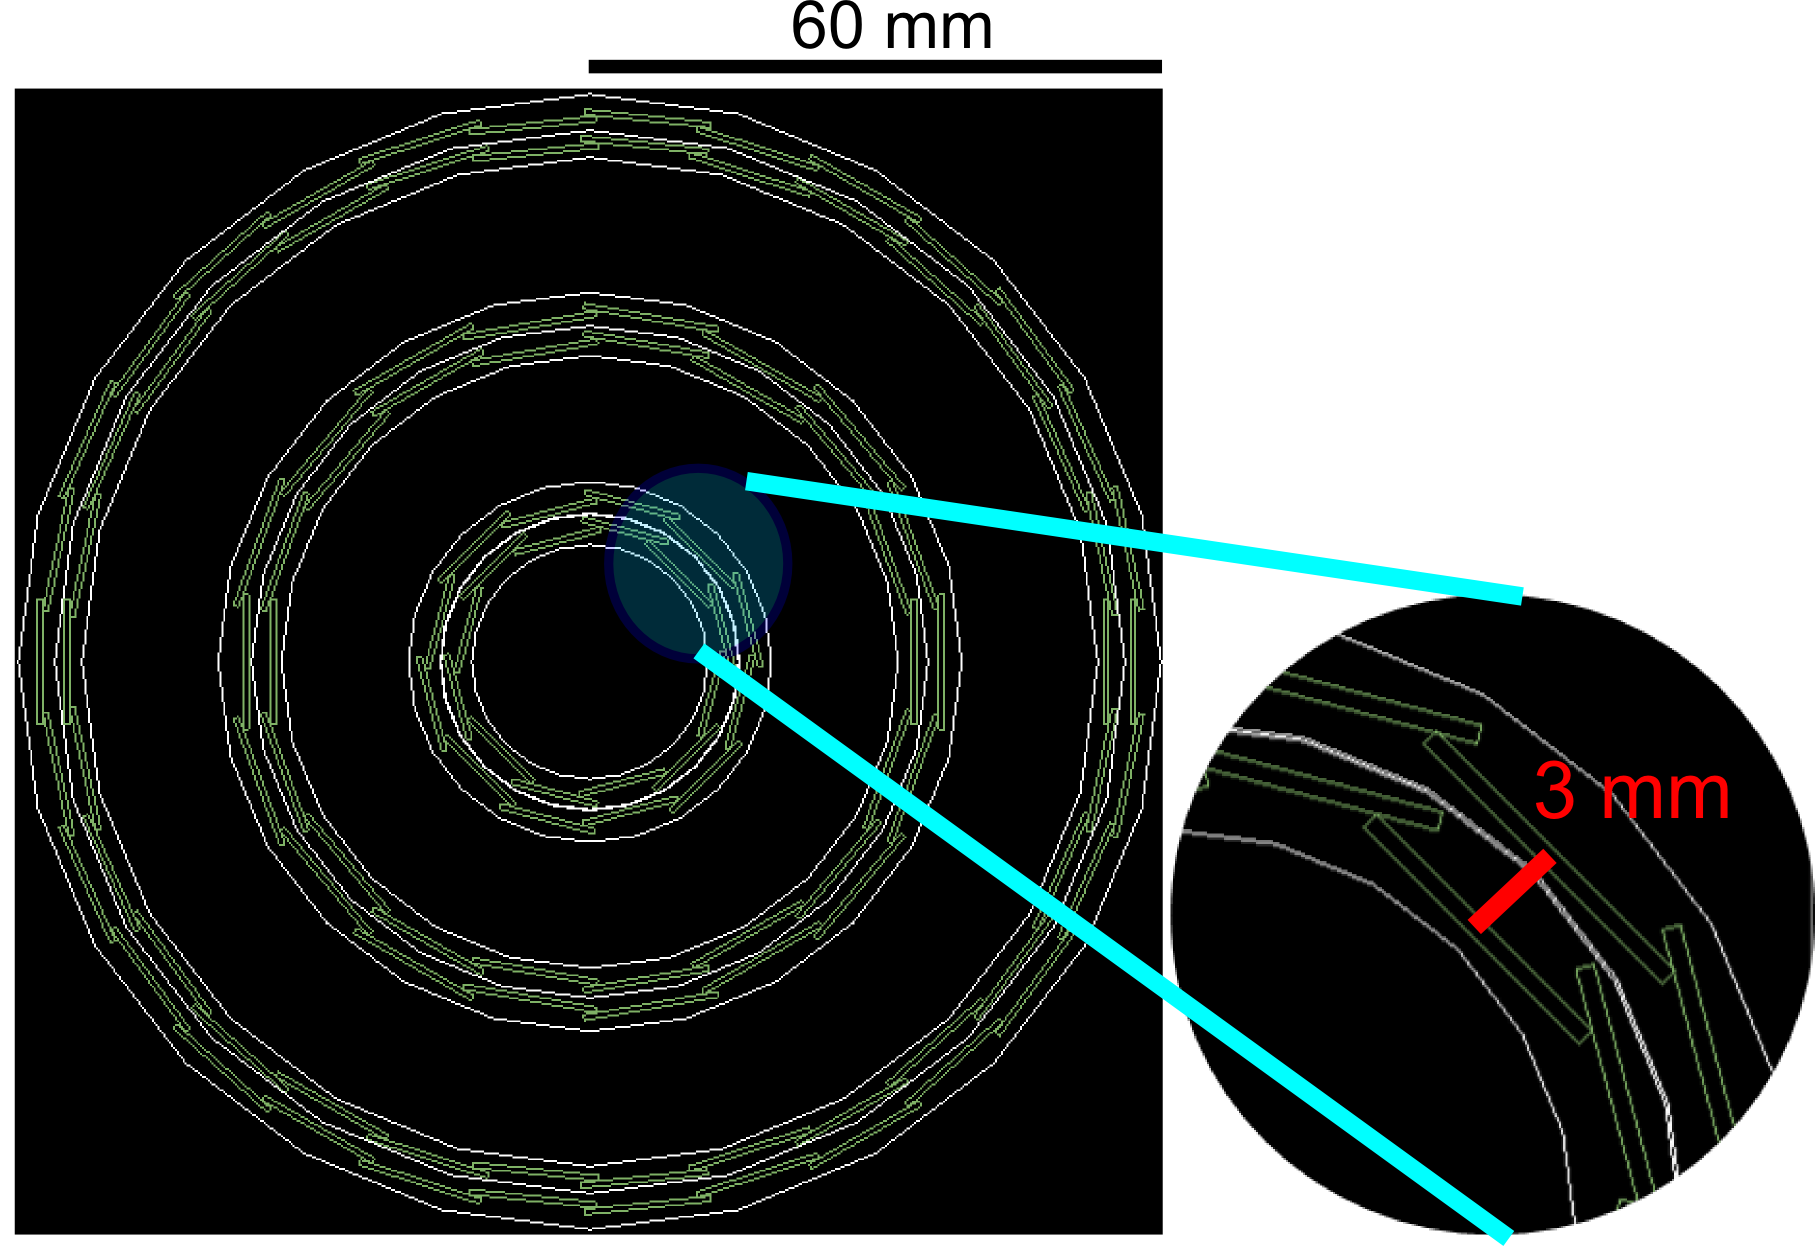
\includegraphics{det_vtxbar_3doublet_barrel3.png}
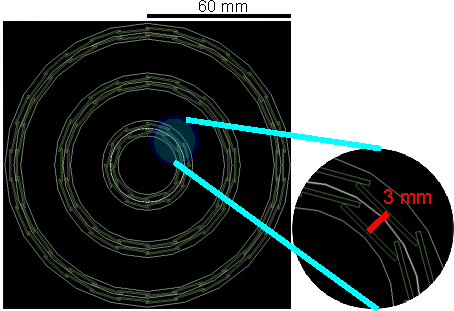
\includegraphics{DoubletVertexFinal_withVolumesAndDetail.pdf}
\subcaption{Modified Geometry Barrel}\label{fig:modifiedbarrel}
\end{minipage}
\caption{View of the r$\phi$ plane (a) Sidloi3's vertex barrel and
(b) the modified barrel. The green boxes depict
individual detector modules. The white lines surrounding each layer depict the detector envelopes as defined 
in SLIC. The detail in (a) shows, to scale, the various material
thicknesses of the module used in the vertex barrels. Every module in both vertex barrels
share the same material budget. Note that the detail in (a) is only to scale in the vertical dimension, not longitudinally.}
\label{fig:barrels}
\end{figure}
\begin{table}
\begin{center}
\begin{small}
	\begin{tabular}{cc||cc}
		\textbf{Detector} & \textbf{Layer} & \textbf{Radius} (mm) & \textbf{Module Dimensions} (mm) \\
		\hline \hline
		\textbf{Sidloi3} & \textbf{1} & 15.05 & 9.6 $\times$ 125.0 $\times$ 0.873 \\
		 & \textbf{2} & 23.03 & 13.8 $\times$ 125.0 $\times$ 0.873 \\
		 & \textbf{3} & 35.79 & 13.8 $\times$ 125.0 $\times$ 0.873 \\
		 & \textbf{4} & 47.50 & 13.8 $\times$ 125.0 $\times$ 0.873 \\
		 & \textbf{5} & 59.90 & 13.8 $\times$ 125.0 $\times$ 0.873 \\
		\hline
		\textbf{Modified Detector} & \textbf{1} & 15.05 & 9.6 $\times$ 125.0 $\times$ 0.873 \\
		 & \textbf{2} & 18.05 & 10.6 $\times$ 125.0 $\times$ 0.873 \\
		 & \textbf{3} & 35.79 & 13.8 $\times$ 125.0 $\times$ 0.873 \\
		 & \textbf{4} & 38.79 & 14.8 $\times$ 125.0 $\times$ 0.873 \\
		 & \textbf{5} & 56.90 & 13.8 $\times$ 125.0 $\times$ 0.873 \\
		 & \textbf{6} & 59.90 & 13.8 $\times$ 125.0 $\times$ 0.873 \\
	\end{tabular}
\caption{Comparison of the geometry specifications for the vertex barrel of Sidloi3 (figure~\ref{fig:sidloi3barrel} and the modified detector (figure~\ref{fig:modifiedbarrel}). The modified detector has a 3~mm gap in radius between layers 1 and 2, 3 and 4, and 5 and 6. In the modified detector, the module width increases by  1~mm in layers 2 and 4. Also notice that the thickness (0.873~mm) and depth in $z$ (125.0~mm) remains the same in both detectors.}
\label{tab:vertexGeom}
\end{small}
\end{center}
\end{table}

\begin{figure}
\begin{minipage}{.5\textwidth}
\centering
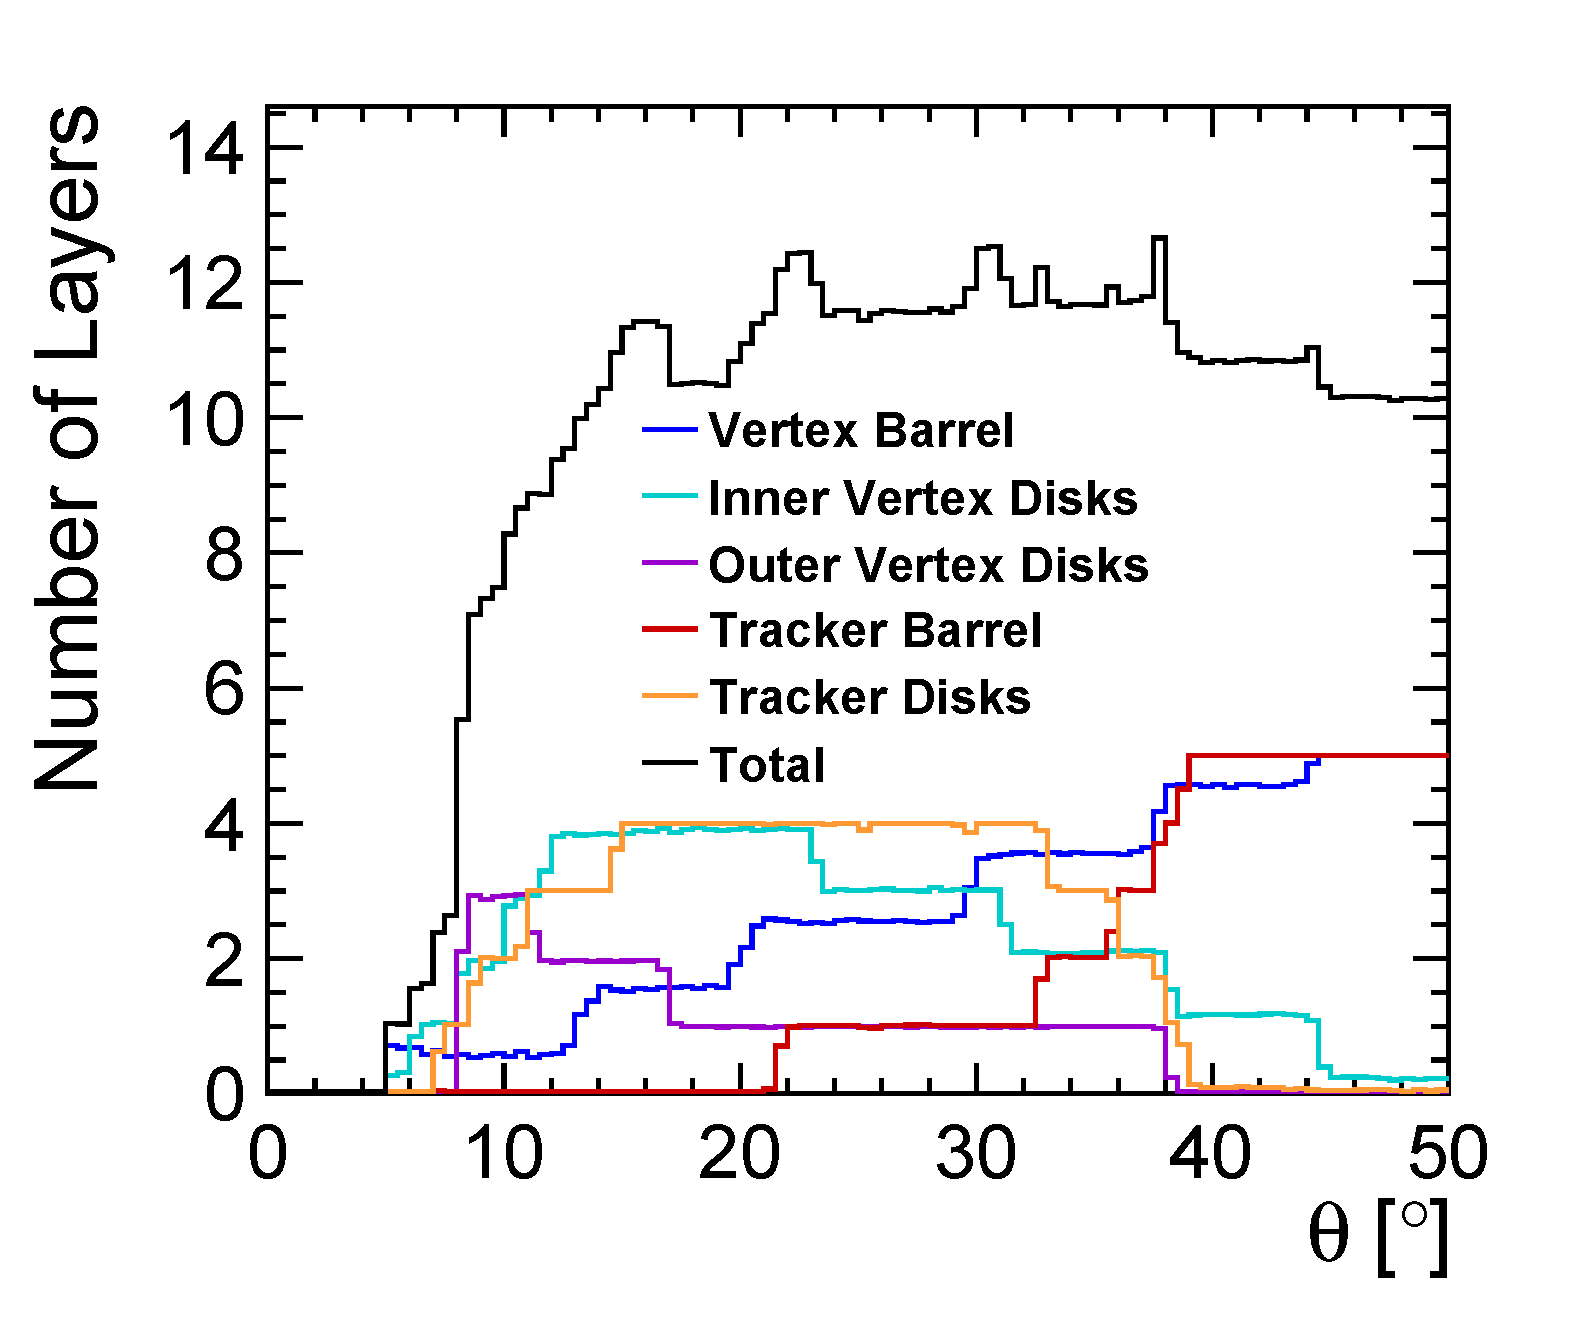
\includegraphics[width=\textwidth]{trackerCoverage_sidloi3.png}
\subcaption{Sidloi3 Coverage}\label{fig:coveragea}
\end{minipage}%
\begin{minipage}{.5\textwidth}
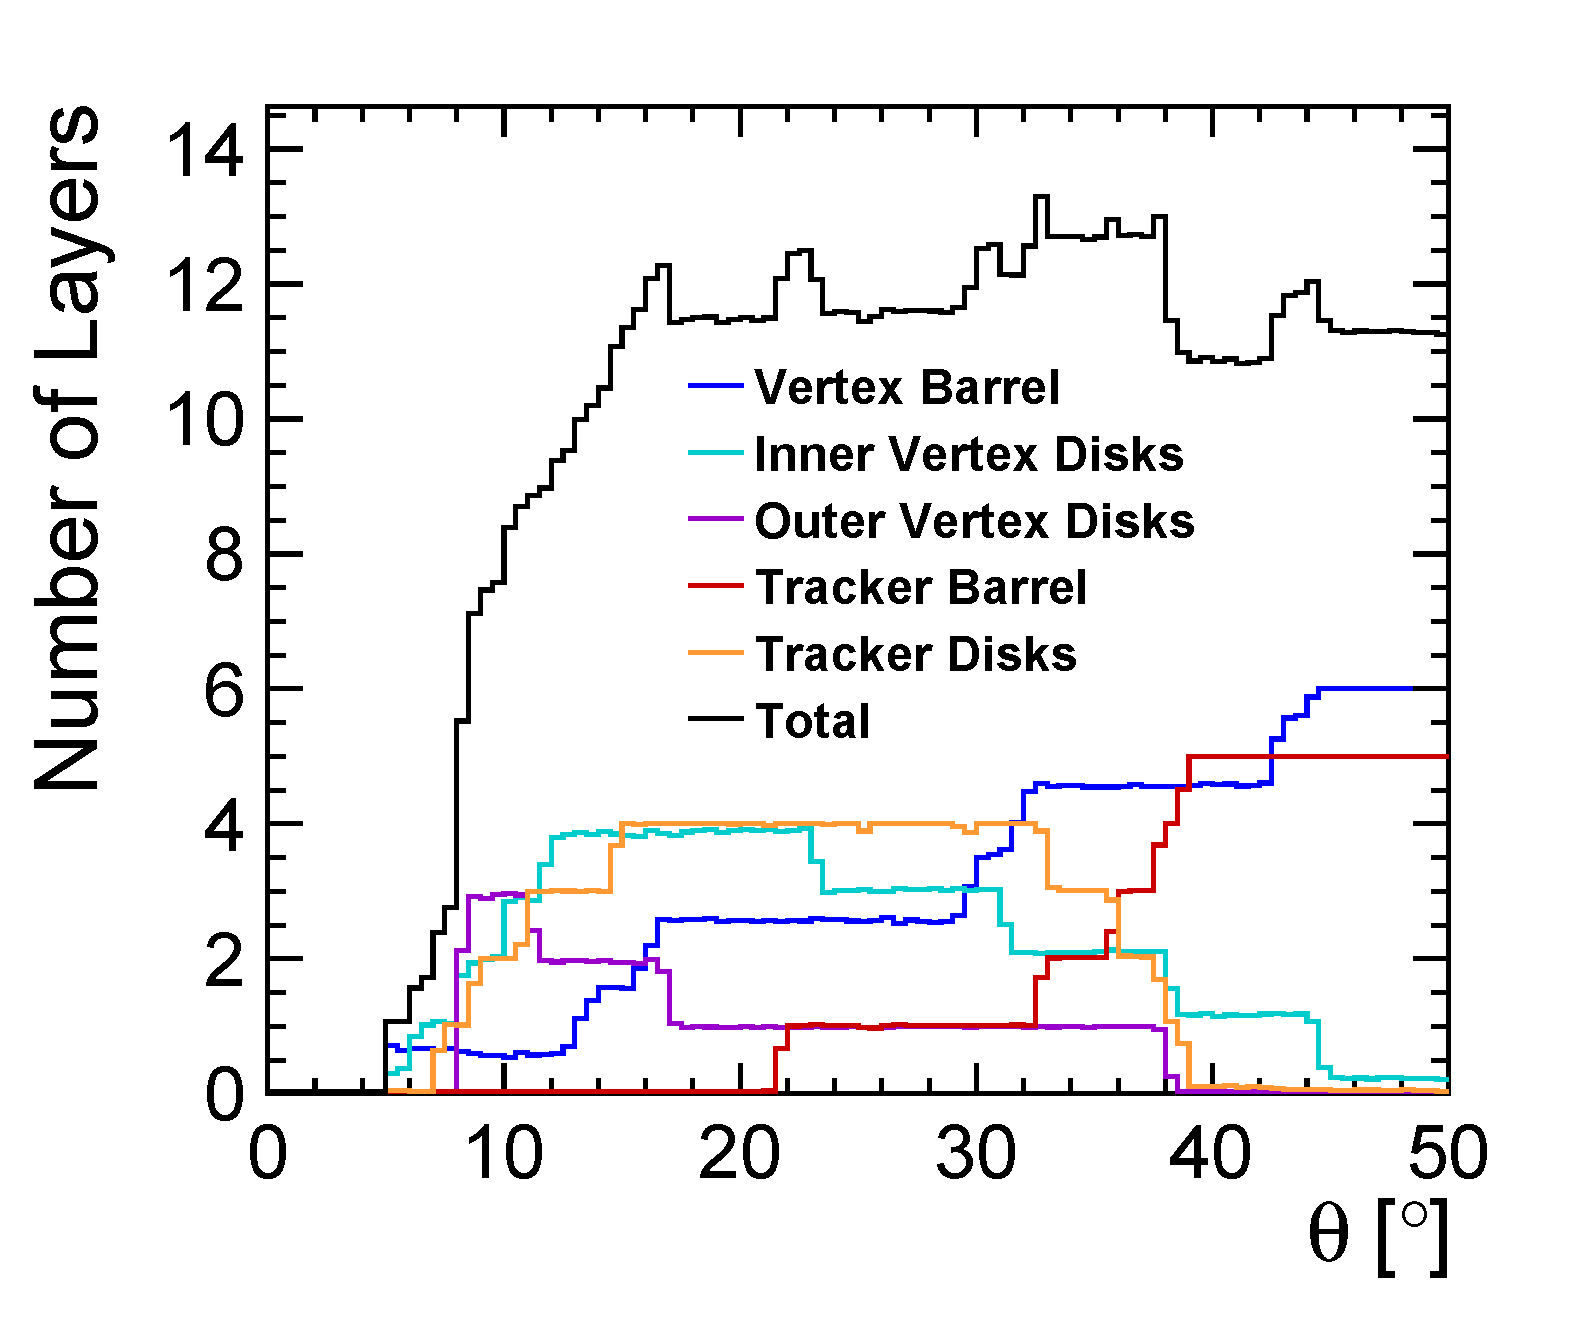
\includegraphics[width=\textwidth]{trackerCoverage_det_vtxbar_3doublet.png}
\subcaption{Modified Geometry Coverage}\label{fig:coverageb}
\end{minipage}
\caption{Coverage of the tracking systems as a function of polar angle for (a) Sidloi3 and (b) the modified detector.
Comparison of the figures illustrates the difference in the coverage of the vertex barrel.
Most noticeably, for high polar angles, the vertex barrel reaches a peak of six layers in the modified geometry as expected,
whereas Sidloi3 reaches a peak of five layers. Coverage is the same for all other tracking systems.}
\label{fig:coverage}
\end{figure}

\iffalse
\begin{figure}
	\centering
	\subfloat[][]{{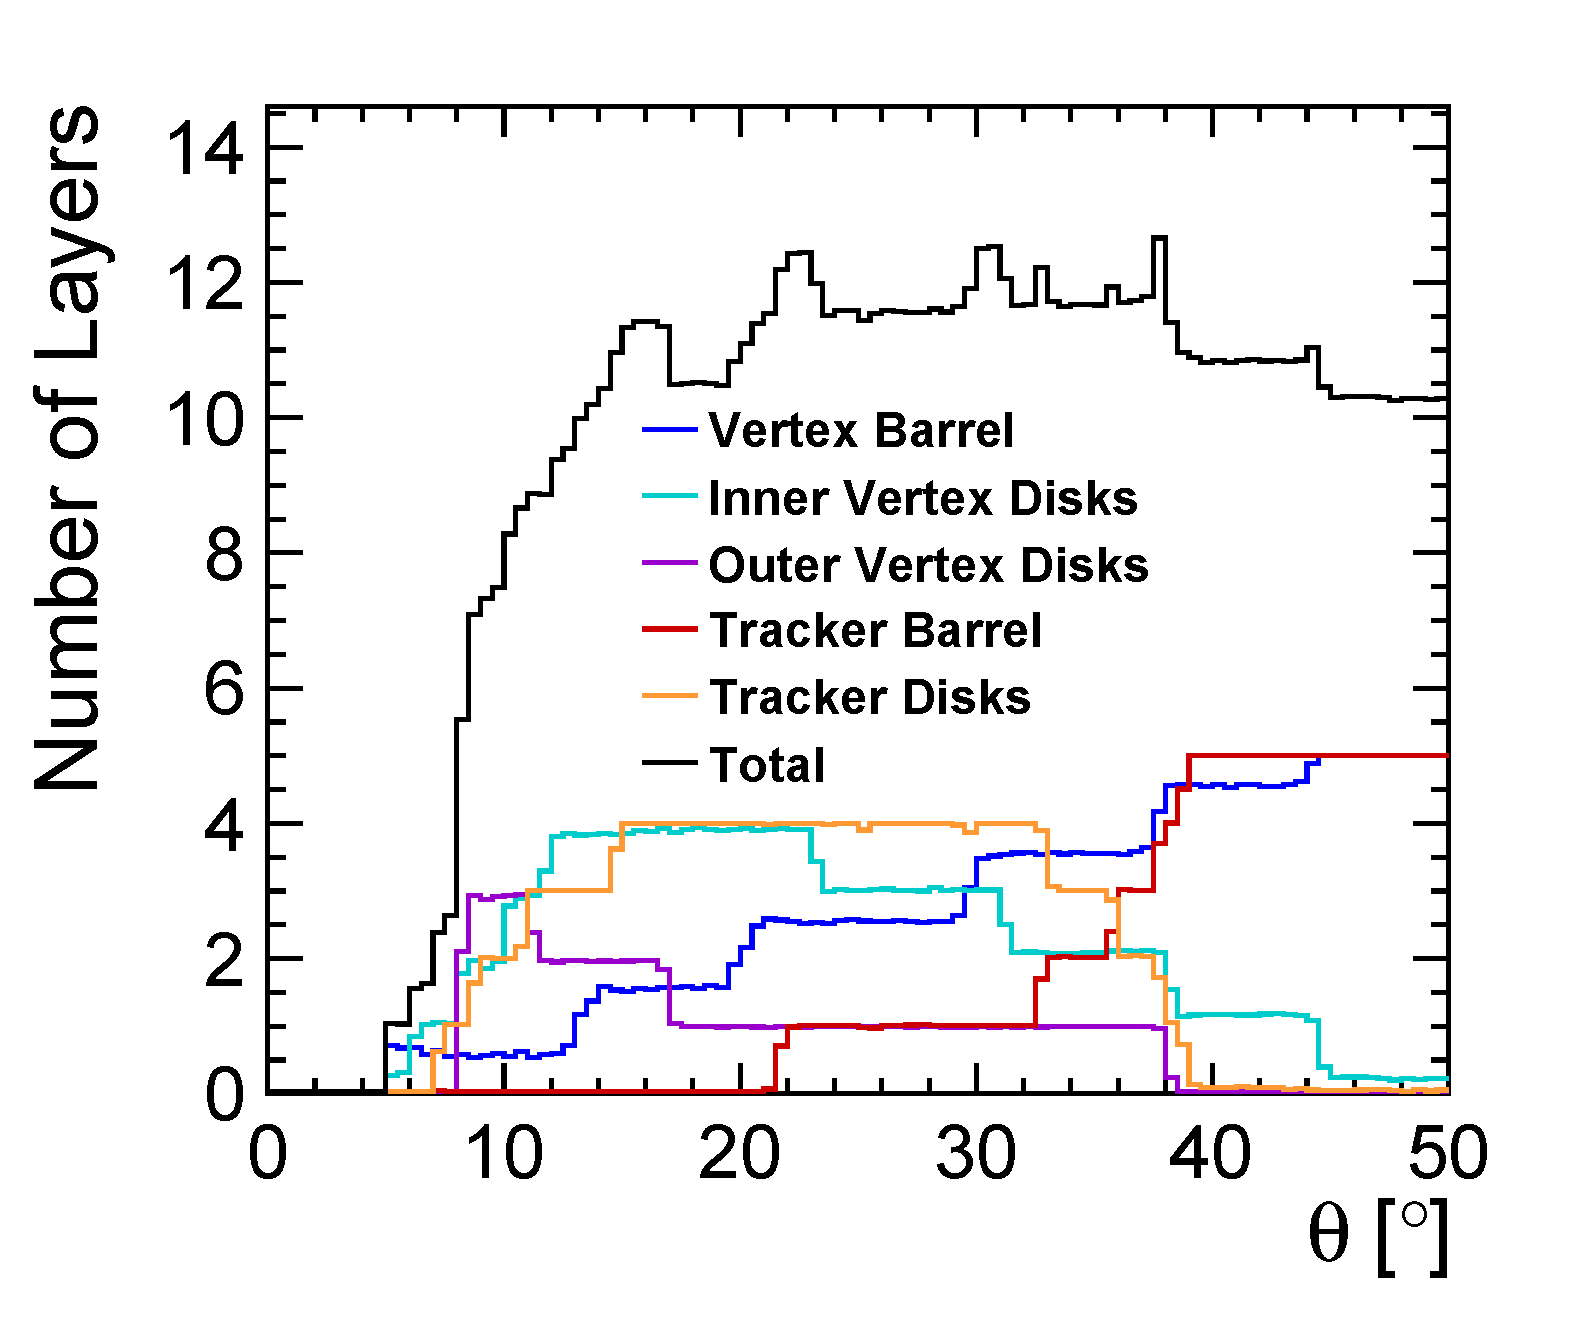
\includegraphics[width=3.0in]{trackerCoverage_sidloi3.png} }}%
	%\parbox{3.0in}{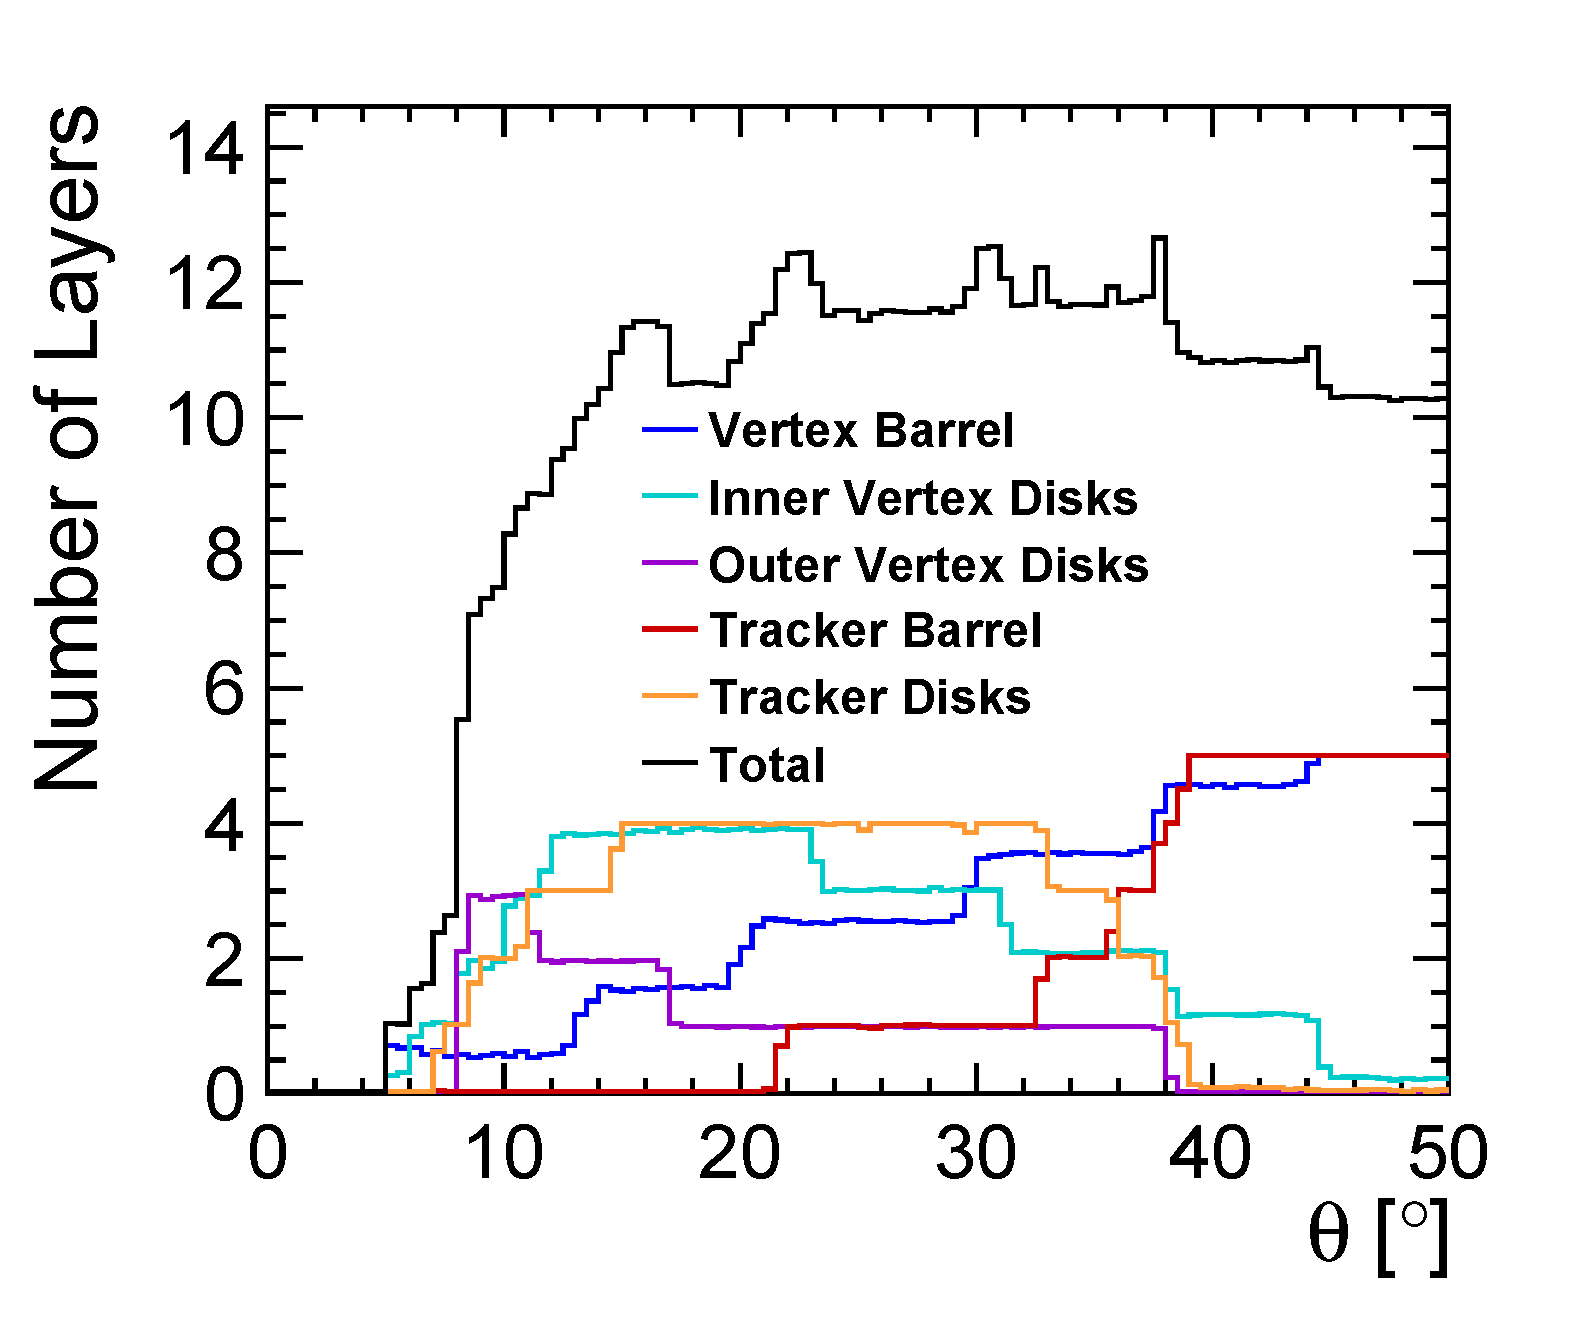
\includegraphics[width=3.0in]{trackerCoverage_sidloi3.png}}
	\caption{Sidloi3 Coverage}
	\qquad
	%\begin{minipage}{3.0in}{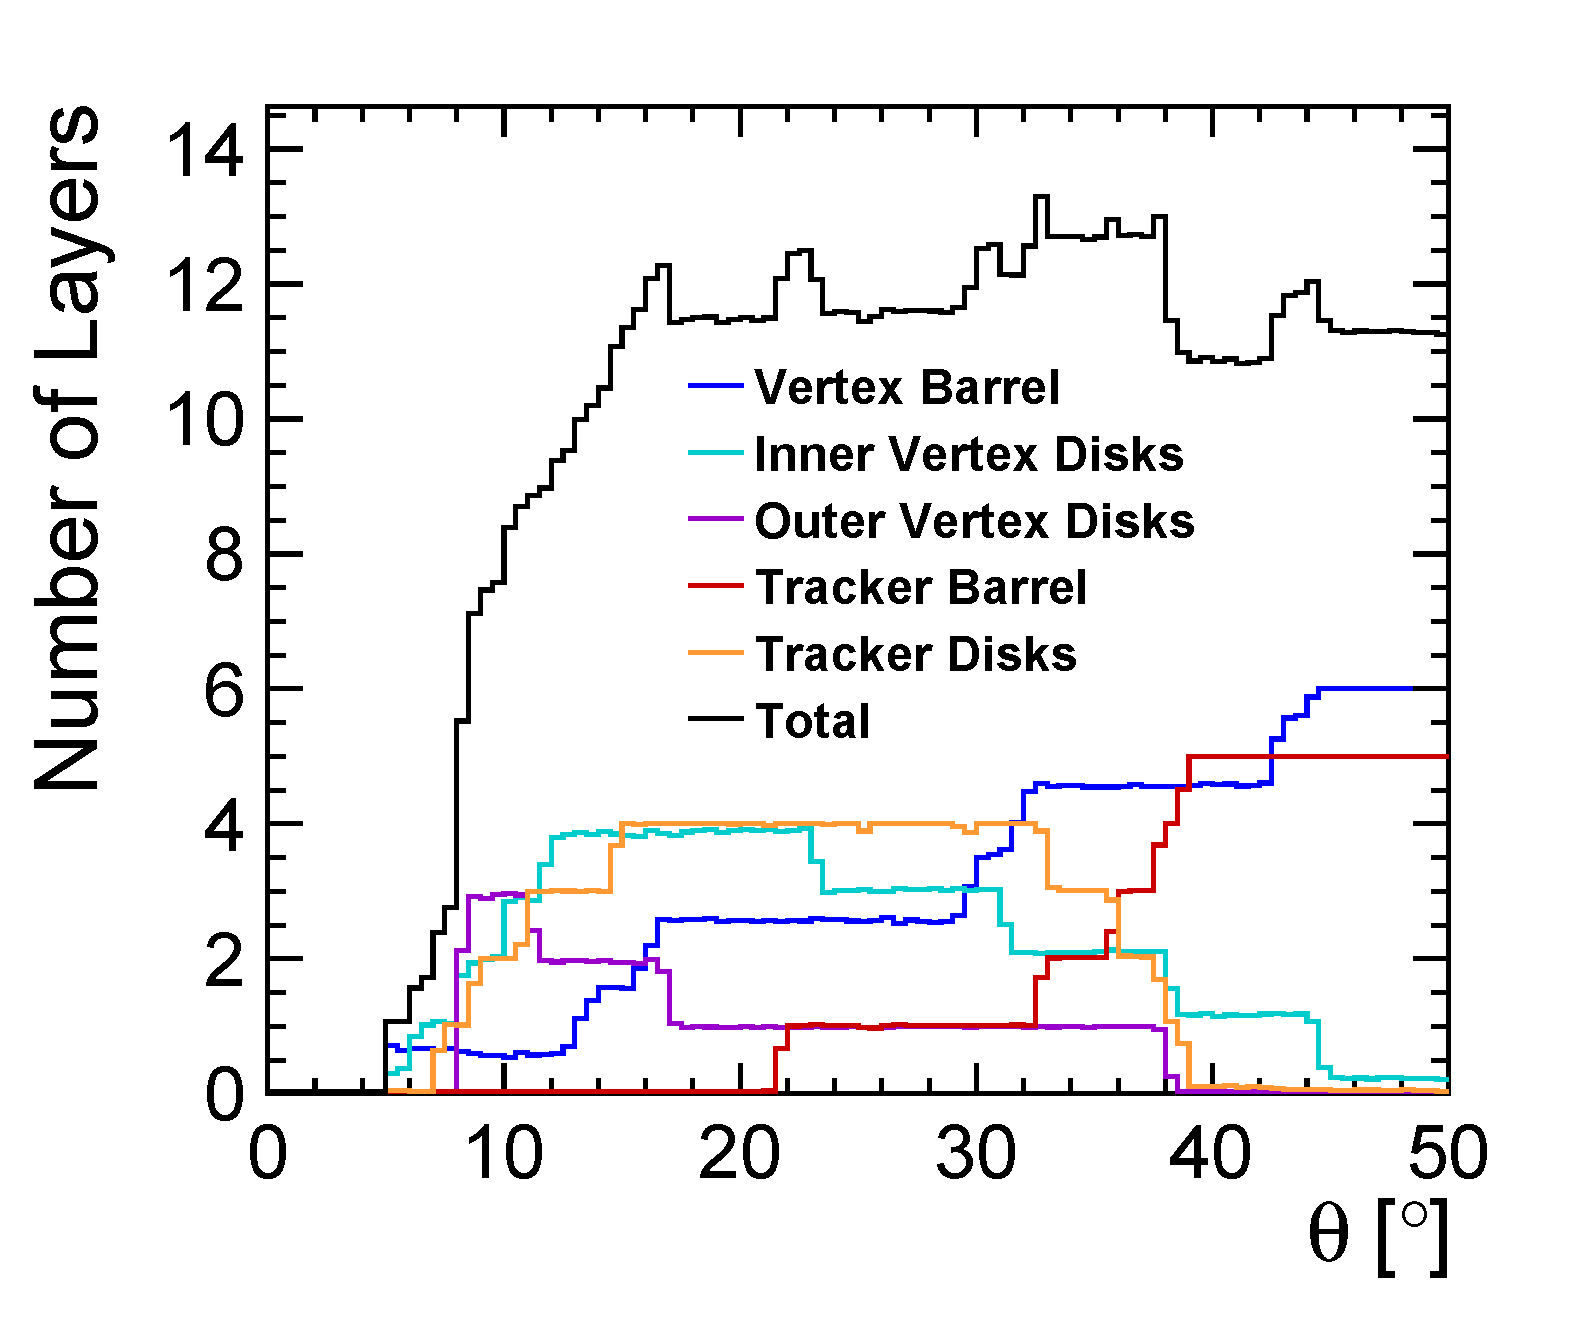
\includegraphics[width=3.0in]{trackerCoverage_det_vtxbar_3doublet.png}}
 	\subfloat[][]{{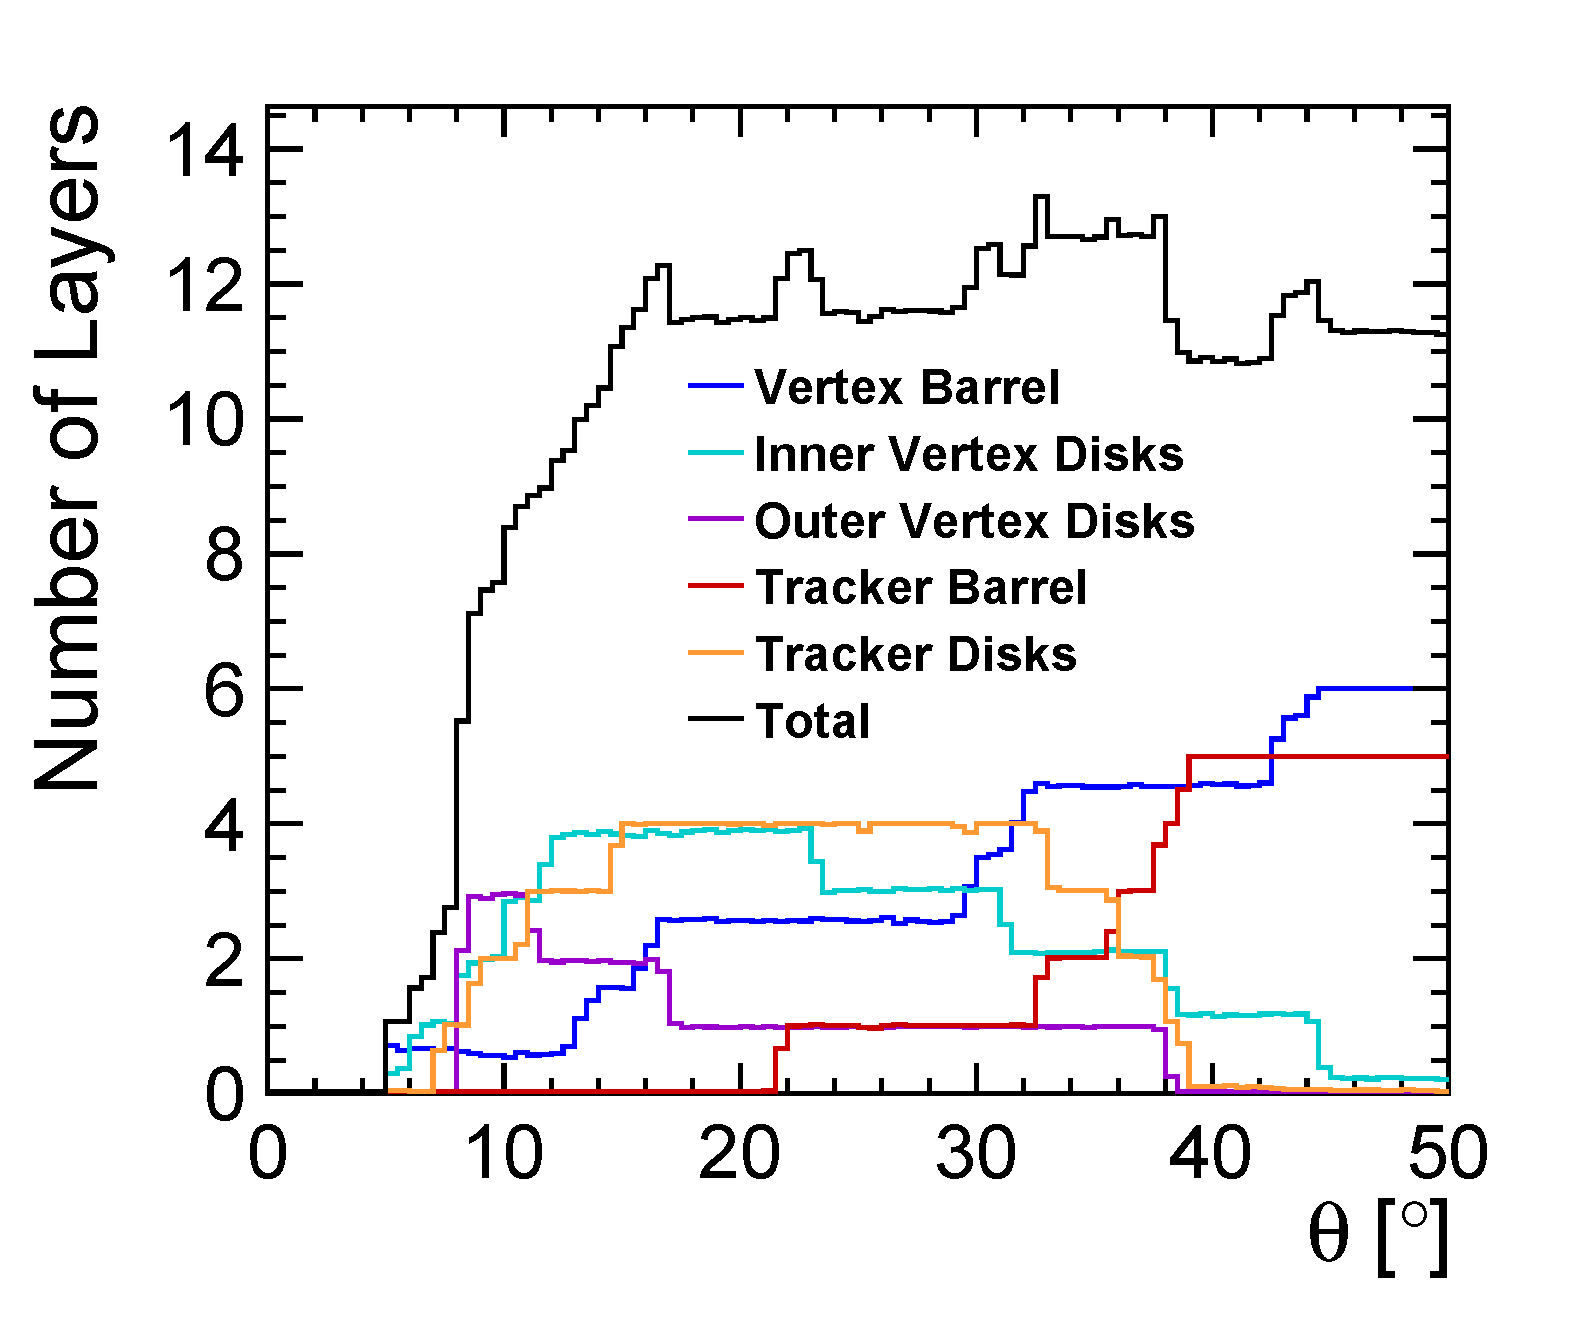
\includegraphics[width=3.0in]{trackerCoverage_det_vtxbar_3doublet.png} }}%
	\caption{Modified Geometry Coverage}
	%\end{minipage}
\caption{Coverage of the tracking systems of both detectors as a function of polar angle. Comparison of the figures illustrates the difference in the coverage of the vertex barrel. Most noticeably, for high polar angles, the vertex barrel reaches a peak of six layers in the modified geometry as expected, whereas Sidloi3 reaches a peak of five layers. Coverage is the same for all other tracking systems.}
\label{fig:coverage}
\end{figure}
\fi

\iffalse
\begin{figure}
\centering
\begin{subfigure}[b]{.5\textwidth}
  \centering
  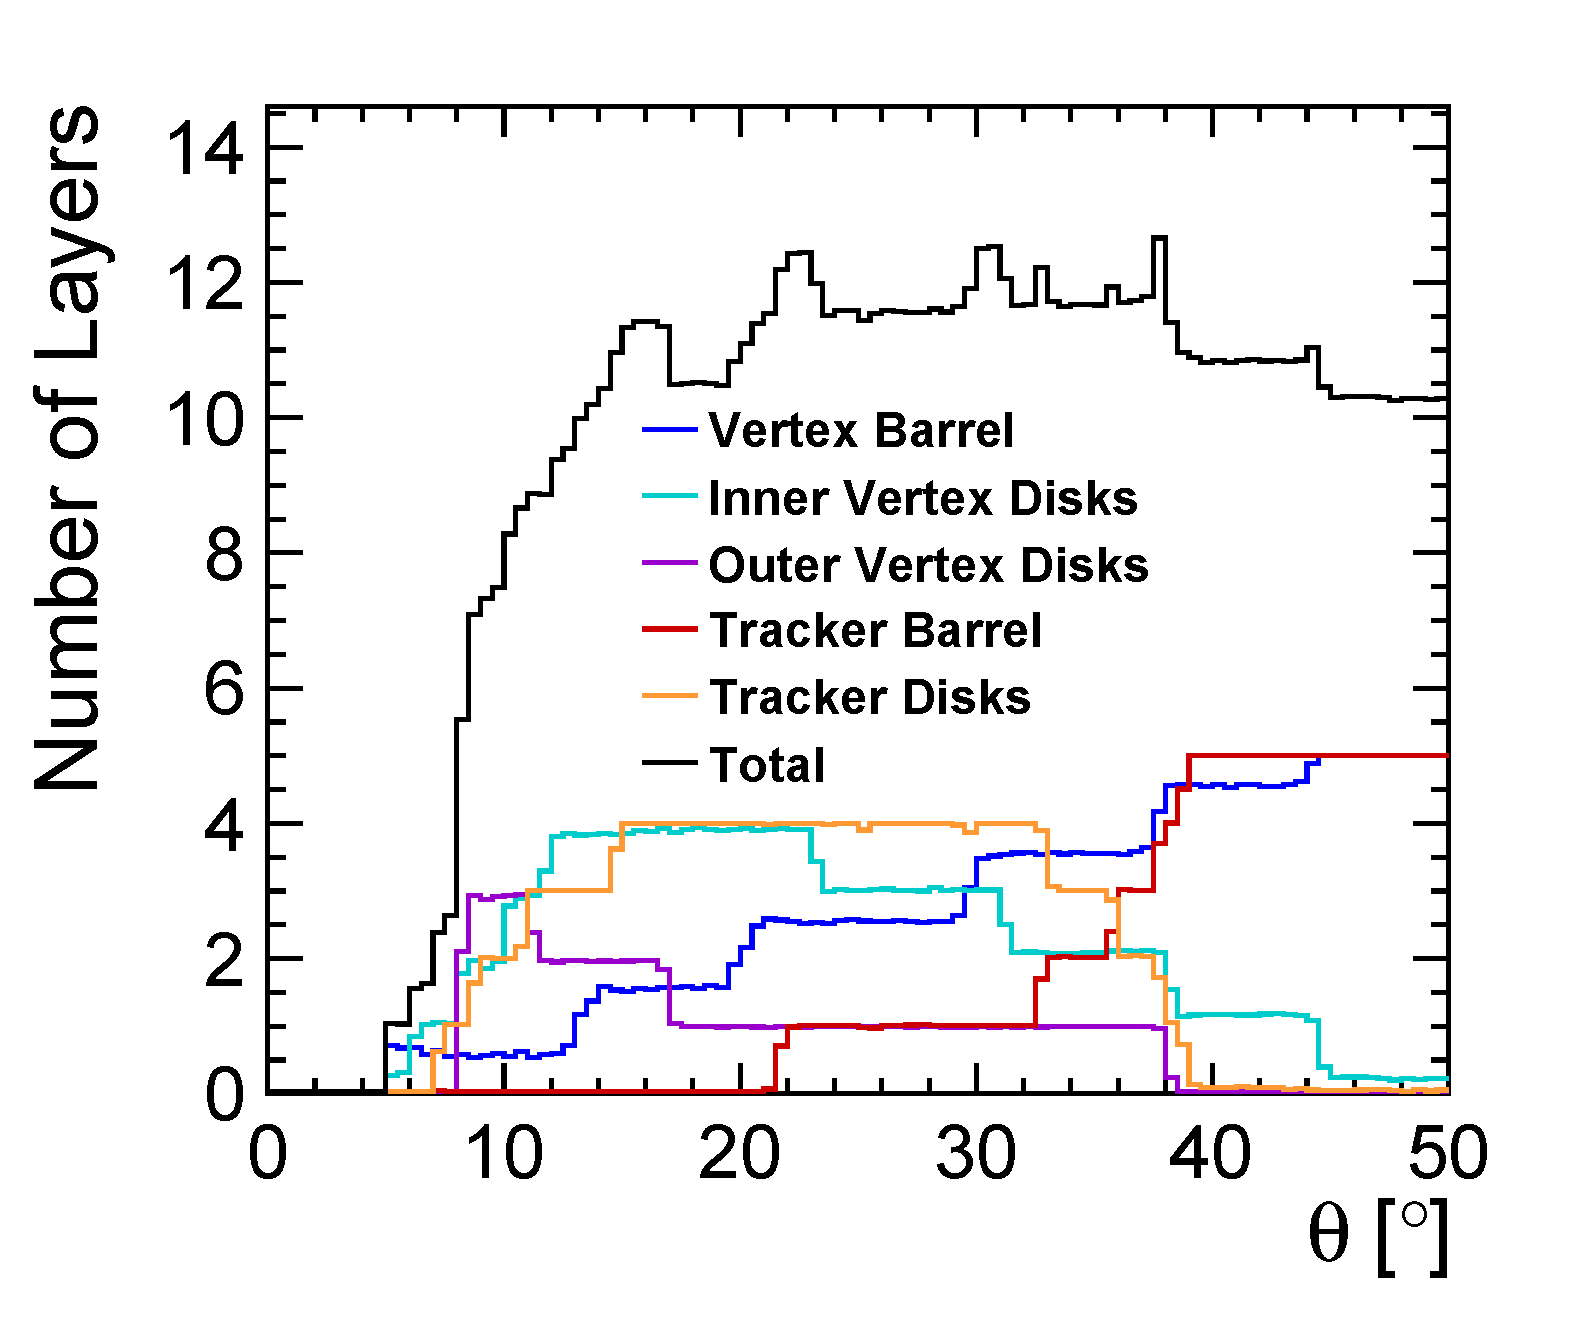
\includegraphics[width=.97\linewidth]{trackerCoverage_sidloi3.png}
  \caption{Sidloi3 Coverage}
  \label{fig:sidloi3Coverage}
\end{subfigure}%
\begin{subfigure}[b]{.5\textwidth}
  \centering
  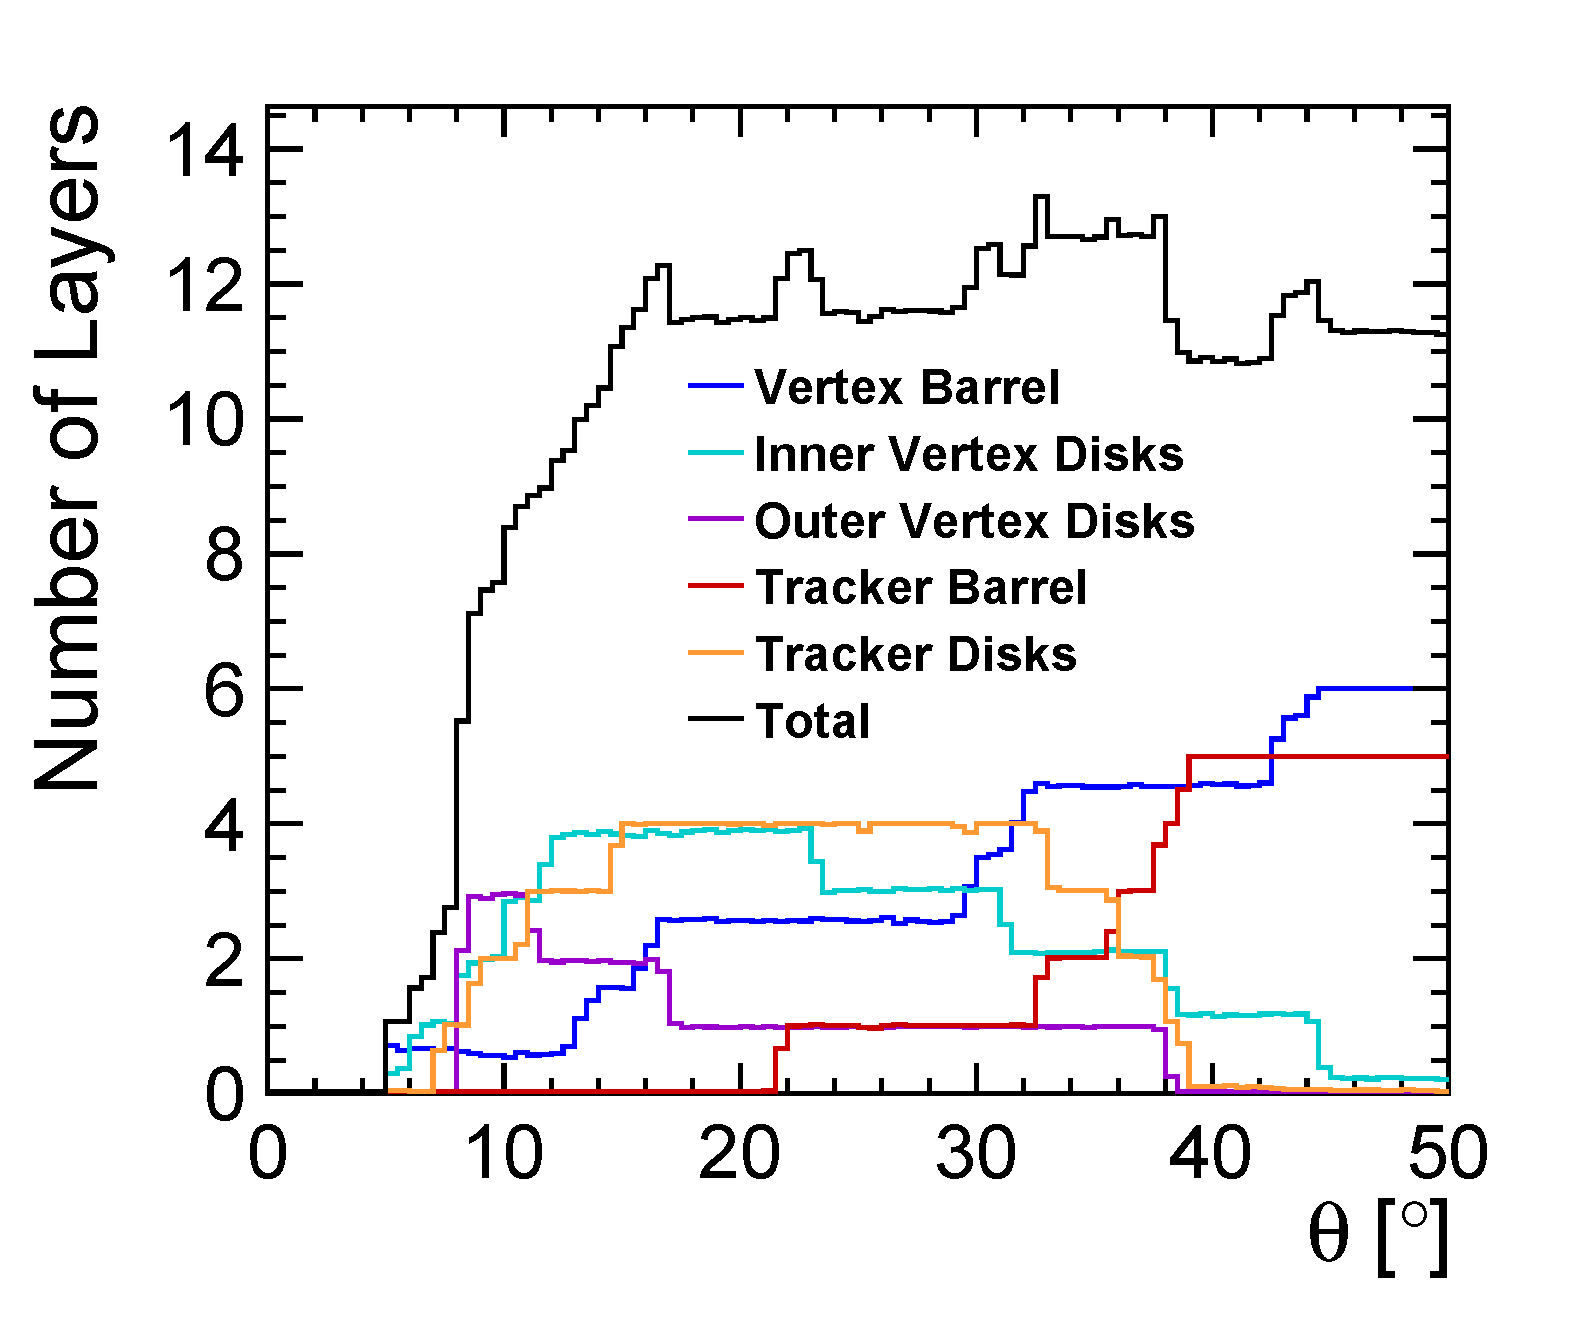
\includegraphics[width=.97\linewidth]{trackerCoverage_det_vtxbar_3doublet.png}
  \caption{Modified Geometry Coverage}
  \label{fig:newDetCoverage}
\end{subfigure}
\caption{Coverage of the tracking systems of both detectors as a function of polar angle. Comparison of the figures illustrates the difference in the coverage of the vertex barrel. Most noticeably, for high polar angles, the vertex barrel reaches a peak of six layers in the modified geometry as expected, whereas Sidloi3 reaches a peak of five layers. Coverage is the same for all other tracking systems.}
\label{fig:coverage}
\end{figure}
\fi